%Katerina Muskova (xmusko00)
%2019, Duben

\documentclass[11pt, a4paper]{article}
\usepackage[left=2cm,text={17cm, 24cm},top={3cm}]{geometry}

\usepackage[czech]{babel}
\usepackage[utf8]{inputenc}
\usepackage[T1]{fontenc}
\usepackage{times}

\usepackage{blindtext}
\usepackage{hyperref}
\usepackage{csquotes}

\usepackage{multirow}
\usepackage{algorithmic}
\usepackage{graphics}
\usepackage{picture}
\usepackage{epsf}
\usepackage{epstopdf}
\usepackage{pdflscape}

\usepackage{titlesec}

\setcounter{secnumdepth}{4}


%$\PassOptionsToPackage{hyphens}{url}
%\usepackage{hyperref}

%\usepackage{url}
%\usepackage{breakurl}

\usepackage{xurl}

\usepackage{flafter}

\begin{document}

%%%%%%%%%%%%%%%%%%%%%%%%%%%%%%% TITLE %%%%%%%%%%%%%%%%%%%%%%
\begin{titlepage}

\begin{center}
	\Huge \textsc{Vysoké učení technické v~Brně}\\
	\huge \textsc{Fakulta informačních technologií}\\
		
	\vspace{\stretch{0.3}}
	\huge Databázové systémy \\
	\huge 2019/2020\\

	\bigskip 
	\bigskip 
	\huge KLUB ANONYMNÍCH ALKOHOLIKŮ
	\vspace{\stretch{0.6}}
\end{center}

{\Large \today \hfill xnosko05, xmusko00}
\end{titlepage}

%%%%%%%%%%%%%%%%%%%%%%%%%%%%%%% DOCUMENT %%%%%%%%%%%%%%%%%%%

\section{Zadání}
Navrhněte informační systém, který bude podporovat anonymní alkoholiky k organizaci sezení
a evidenci vypitého alkoholu. Systém uchovává základní informace o alkoholicích, jako je
jejich věk, pohlaví, patrony, kteří je podporují a se kterými se nepravidelně scházejí na různých
místech a v různých datech a rovněž i informace o odbornících, kteří na ně lékařsky dohlíží.
Odborníci musí mít patřičnou expertízu pro pečování o alkoholiky, a mít minimální lékařskou
praxi, která je v systému evidována. Patronem však může být kdokoliv. Pravidelně se konají
sezení, kterých se účastní až dvanáct alkoholiků a navíc můžou být přítomni jak patroni tak i
odborníci a dohlížet nad diskuzí. U každého sezení nás zajímá datum, čas, a místo konání.
Těchto míst je pouze několik oficiálních a dedikovaných. Každé sezení je vedeno jednou
osobou. Neformální schůzky s patrony však mohou být organizovány v libovolné lokalitě.
Alkoholici se musí alespoň třikrát ročně účastnit nějakého sezení, a v případě, že se více jak tři
měsíce nedostaví na žádné sezení je jim systémem zaslána upomínka. U alkoholiků jsou
pravidelně (i nepravidelně a nečekaně) prováděny kontroly odborníky, na kterých se měří míra
alkoholu v jejich krvi. Tato míra vypitého alkoholu je pak evidována do systému, rovněž s
původem a typem vypitého alkoholu. Alkoholici však mohou sami zaevidovat (ze špatného
svědomí), že alkohol požili (tedy mimo prováděné kontroly) a tuto informaci rovněž přidat do
systému.

\section{ER diagram}

\begin{figure}[ht]
	\begin{center}
	\scalebox{0.5}{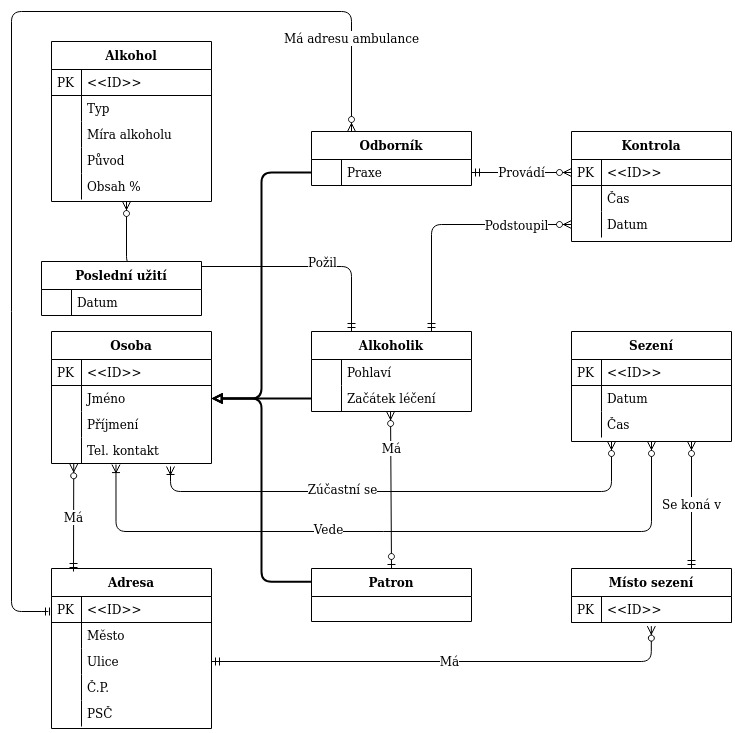
\includegraphics{obr/IDS_ERD.jpg}}
	\caption{ERD}
	\end{center}
\end{figure}

\section{UC diagram}

\begin{figure}[ht]
	\begin{center}
	\scalebox{0.6}{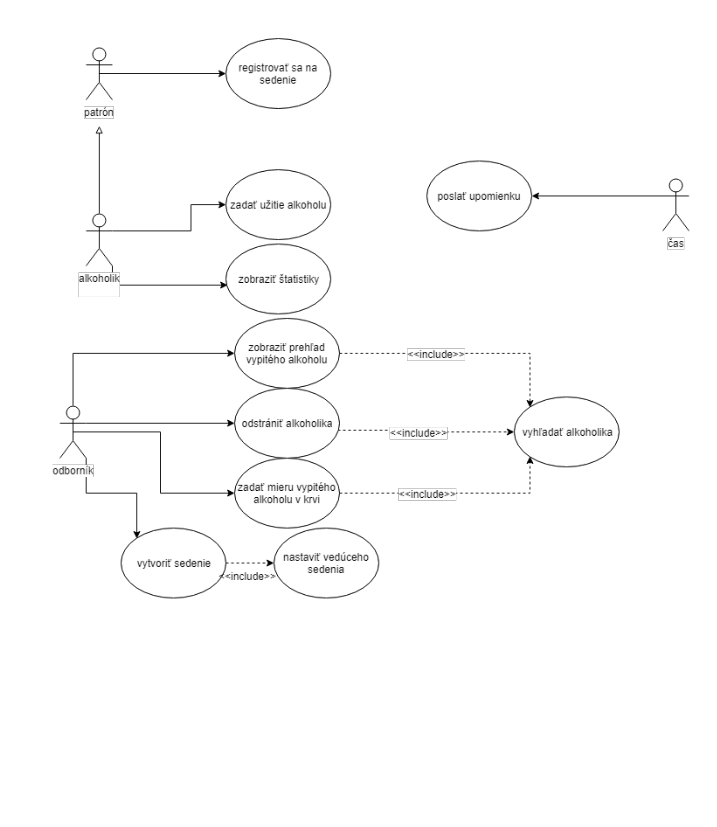
\includegraphics{obr/IDS_UCD.png}}
	\caption{UCD}
	\end{center}
\end{figure}

 \newpage

\section{Návrh databáze}

\begin{figure}[ht!]
	\begin{center}
	\rotatebox{270}{\scalebox{0.5}{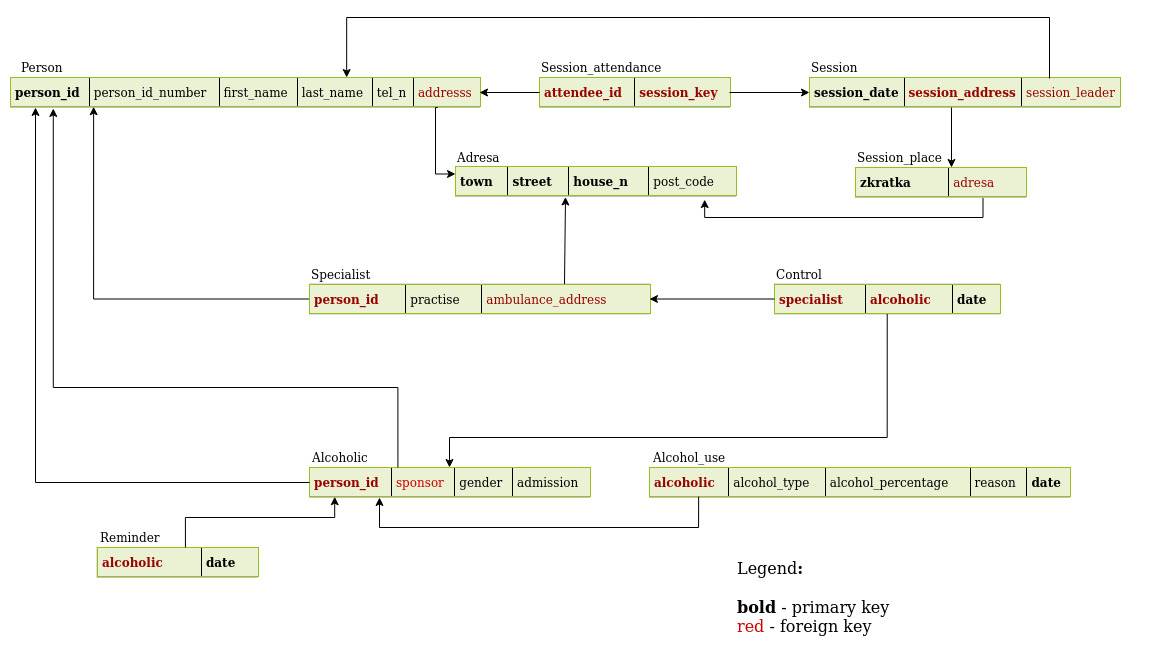
\includegraphics{obr/IDS_Tables.jpg}}}
	\caption{DB}
	\end{center}
\end{figure}

 \newpage

\section{Implementace}
\subsection{Generalizace - Specializace}
Generalizaci specializaci jsme využily u vztahu \texttt{osoba} $\leftarrow$ \texttt{alkoholik, specialista, sponzor}.\\
Máme zde jednu tabulku pro nadtyp \texttt{osoba} a tři tabulky pro podtypy.

\subsection{Trigger}
Všechny trigey jsou spuštěny pří vložení, nebo modifikaci řádku.

\subsubsection*{Check\_person\_id\_number}
Tento trigger kontroluje zadaný formát rodného čísla osoby v tabulce \texttt{PERSON}.
Konkrétně podle délky, roku, dne, měsíce a dělitelnosti jednácti.\\
V případě špatného formátu je vyhozena chyba číslo -20001.

\subsubsection*{Check\_session\_collision}
Trigger konrolující kolize sezení v tabulce \texttt{SESSION}.\\
Za kolizi se považuje sezení, které má stejné místo a datum se liší maximálně o hodinu.
Pokud nastane kolize, je vyhozena chyba číslo -20001.

\subsubsection*{Generate\_user\_id}
Trigger na autoinkrementaci jsme použili u tabulky Person, který má stejnou funkci jako  \texttt{GENERATED AS IDENTITY NOT NULL} - generuje počínaje jedničkou unikátní ID.\\

\subsection{Procedury}

\subsubsection*{Count\_alcoholics\_at\_session (p\_session\_name number)}
Dle zadání je maximální počet alkoholiků na sezení dvanáct. Tato procedura tiskne počet alkoholiků příhlášených na daném sezení \texttt{(p\_session\_name)}. Pokud sezení není nalezeno, vytiskne se "Session has not been found."

\subsubsection*{Add\_reminder (p\_months\_num number)}
V zadání je specifikováno, že pokud se alkoholik nezůčastní sezení tři měsíce, má mu být zaslána upomínka. K vytvoření upomínek právě slouží tato procedura.\\

U každého alkoholika se zkontroluje, zda v posledních n měsících \texttt{(p\_months\_num)} navštívil sezení. Pokud ne, je vygenerována nová upomínka.

\subsection{Indexy}
Ke každé tabulkce jsme přidaly indexy na primární klíče. Podle primárních klíčů se totiž většinou v tabulkách vyhledává a proto se tímto vyhledávání urychlí.

\subsection{EXPLAIN PLAN}
V našem kódu explain plan zobrazuje sekvenci aperací u příkazu \texttt{SELECT} přes dvě tabulky.

Select zobrazí seznam alkoholiků, kteří požili alkohol a zároveň kolikrát sa to stalo. Po vytvoření indexu \texttt{alcohol\_use\_i} by mělo být vyhladávaní rychlejší. 

\begin{table}[h]
	\begin{tabular}{r r l c c c c c}
	 & ID & Operation & Name & Rows & Bytes &  Cost  & Time & \hline \\
	 & 0 & SELECT STATEMENT 	& & 1 & 18 & 6 (34) & 00:00:01\\
	 & 1 & SORT ORDER BY     	& & 1 & 18 & 6 (34) & 00:00:01\\
	 & * 2 & FILTER 				& &  &  &  & \\
	 & 3 & HASH GROUP BY 		& & 1 & 18 & 6 (34) & 00:00:01\\
	 & 4 & NESTED LOOPS    		& & 1 & 18 & 4  & 00:00:01\\
	 & 5 & NESTED LOOPS    		& & 1 & 18 & 4  & 00:00:01\\
	 & 6 & TABLE ACCESS FULL   	& ALCOHOL\_USE & 1 & 3 & 3  & 00:00:01\\
	 & * 7 & INDEX UNIQUE SCAN  	& SYS\_C001168092 & 1 & 0 & 0  & 00:00:01\\	
	 & 8 & TABLE ACCESS BY INDEX ROWID	& PERSON & 1 & 15 & 1  & 00:00:01\\ 
	\end{tabular}
	
	\vspace{2em}
	
	\begin{tabular}{r r l c c c c c}
	 & ID & Operation & Name & Rows & Bytes &  Cost  & Time & \hline \\
	 & 0 & SELECT STATEMENT 	& & 1 & 18 & 4 (50) & 00:00:01\\
	 & 1 & SORT ORDER BY     	& & 1 & 18 & 4 (50) & 00:00:01\\
	 & * 2 & FILTER 				& &  &  &  & \\
	 & 3 & HASH GROUP BY 		& & 1 & 18 & 4 (50) & 00:00:01\\
	 & 4 & NESTED LOOPS    		& & 1 & 18 & 2  & 00:00:01\\
	 & 5 & NESTED LOOPS    		& & 1 & 18 & 2  & 00:00:01\\
	 & 6 & INDEX FULL SCAN     	& ALCOHOL\_USE & 1 & 3 & 1  & 00:00:01\\
	 & * 7 & INDEX UNIQUE SCAN  	& SYS\_C001168092 & 1 &  & 0    & 00:00:01\\	
	 & 8 & TABLE ACCESS BY INDEX ROWID	& PERSON & 1 & 15 & 1    & 00:00:01\\ 
	\end{tabular}
	
	\vspace{2em}
	
	\begin{tabular}{l l l}
	& 2 & filter(COUNT(*)>0) \\
	& 7 & access(P.PERSON\_ID=AU.ALCOHOLIC)\\
	\end{tabular}
\end{table}

Vyhladánání by se dalo teoreticky jestě urychlit s pomocí materializovaného podledu.

\subsection{Přístupová práva}
Přístupová práva jsme využily pro přístup druhého člena k databázy.

\subsection{Materializovaný pohled}
Materializavaný pohled zabrazuje alkoholiky a jejich počet kontrol.\\
Pohled je vytvořen okamžitě (\texttt{BUILD IMMEDIATE}). \\
Je možné ho aktualizovatpomocí příkazu
(\texttt{DBMS\_MVIEW.REFRESH('alcoholic\_control\_count')}).

\section{Závěr}
Pro přístup k databázi jsme využívali DataGrip od JetBrainu.\\
Projekt se vyplatilo dělat souběžně s přednáškami, protože si člověk hned vyzkoušel probrané učivo v praxi.\\

\section{Zdroje}

\url{https://www.w3schools.com/sql/}\\
\url{https://www.cssz.cz/web/cz/standardni-kontrola-rodneho-cisla-a-evidencniho-cisla-pojistence}\\
\url{https://docs.oracle.com/database/121/index.htm}\\

\end{document}
